\chapter{Diseño del protocolo de control In-Band}
\label{ch:analisis}

En este capítulo, se abordará una fase fundamental del proyecto, centrada en el diseño de un protocolo de control In-Band para la gestión de redes. En este capítulo, se realizará un exhaustivo análisis de soluciones anteriores basadas en el enfoque In-Band, donde se explorarán diferentes propuestas y se evaluarán sus fortalezas y debilidades.\\
\\
El objetivo principal será definir las funcionalidades básicas que debe poseer el protocolo de control In-Band, considerando los requisitos específicos del proyecto y las necesidades de los entornos de redes actuales. Se examinarán aspectos clave, como la capacidad de establecer una conexión entre los nodos de la red y el controlador, el manejo eficiente del plano de datos para la transmisión de información de control y la escalabilidad para adaptarse a entornos de redes heterogéneas y de gran tamaño. Además, se proporcionará una explicación detallada del funcionamiento del protocolo diseñado, describiendo los diferentes componentes, los mensajes intercambiados entre nodos y controlador, así como los procedimientos de configuración y gestión de la red. Se analizarán las decisiones de diseño tomadas y se justificarán en base a los objetivos del proyecto y las características de los entornos de redes abordados.Por último, se tomará una decisión sobre la plataforma más adecuada para la implementación del protocolo de control In-Band. Se evaluarán diferentes opciones, considerando factores como la disponibilidad de herramientas y tecnologías relevantes, la compatibilidad con los requisitos del proyecto y la viabilidad de su implementación en entornos reales.

%%%%%%%%%%%%%%%%%%%%%%%%%%%%%%%%%%%%%%%%%%%%%%%%%%%%%%%%%%%%%%%%%%%%%%%%%%%%%%%%%%%%%%%%%%%%%%%%%
\section{Protocolo In-Band}
\label{sec:ana_inband}

%%%%%%%%%%%%%%%%%%%%%%%%%%%%%%%%%%%%%%%%%%%%%%%%%%%%%%%%%%%%%%%%%%%%%%%%%%%%%%%%%%%%%%%%%%%%%%%%%
\section{Plataforma de desarrollo y validación}
\label{sec:ana_mininet_wifi}

%%%%%%%%%%%%%%%%%%%%%%%%%%%%%%%%%%%%%%%%%%%%%%%%%%%%%%%%%%%%%%%%%%%%%%%%%%%%%%%%%%%%%%%%%%%%%%%%%
\section{Agente \glsentryshort{sdn}}
\label{sec:ana_switch}

%%%%%%%%%%%%%%%%%%%%%%%%%%%%%%%%%%%%%%%%%%%%%%%%%%%%%%%%%%%%%%%%%%%%%%%%%%%%%%%%%%%%%%%%%%%%%%%%%
\section{Agente de control \glsentryshort{sdn}}
\label{sec:ana_controller}

%%%%%%%%%%%%%%%%%%%%%%%%%%%%%%%%%%%%%%%%%%%%%%%%%%%%%%%%%%%%%%%%%%%%%%%%%%%%%%%%%%%%%%%%%%%%%%%%%


%%%%%%%%%%%%%%%%%%%%%%%%%%%%%%%%%%%%%%%%%%%%%%%%%%%%%%%%%%%%%%%%%%%%%%%%%%%%%%%%%%%%%%%%%%%%%%%%%
\section{Análisis de la clase \texttt{UserAP} en Mininet-WiFi}
\label{sec:ana_userap}

En esta sección, vamos a sumergirnos en un análisis exhaustivo de la clase \texttt{UserAP} en Mininet-WiFi, una pieza fundamental que envuelve al \gls{bofus}. Al observar detenidamente el diagrama UML de clases en la figura \ref{fig:userAP}, nos encontramos con una intrigante jerarquía de clases relacionadas con \texttt{UserAP}. En el centro de esta estructura se encuentran las clases primigenias, \texttt{Node} y \texttt{Node\_wifi}, que se llevan la mayor carga lógica al albergar la mayoría de atributos y métodos esenciales. Estas clases primigenias desempeñan un papel crucial al gestionar una serie de operaciones vitales. Entre sus responsabilidades se encuentran la creación de \textit{Network namespaces}, la configuración y creación de interfaces inalámbricas, el manejo del \gls{tc} para establecer los atributos de los enlaces y mucho más. Son el núcleo de la implementación que permite el funcionamiento armonioso de la infraestructura.\\
\\
No obstante, es importante destacar que la clase \texttt{UserAP}, encargada de encapsular al \gls{bofus}, también aporta su propia lógica especializada. Su tarea principal radica en la gestión del proceso \texttt{HostAPd}, un daemon que trabaja incansablemente para materializar las diversas funcionalidades de punto de acceso. Este componente es fundamental para dotar de vida y dinamismo a la red inalámbrica emulada. Además de su papel esencial en el despliegue del \gls{bofus}, estas clases tienen una responsabilidad adicional: implementar una interfaz de ejecución que permite adaptar las condiciones del escenario a los parámetros necesarios de la interfaz de línea de comandos del software switch \gls{sdn}. Esta adaptabilidad se convierte en una ventaja estratégica, ya que proporciona la flexibilidad necesaria para personalizar y ajustar el entorno según las necesidades específicas de cada caso de uso.
\newpage
% fig
\begin{figure}[ht!]
    \centering
    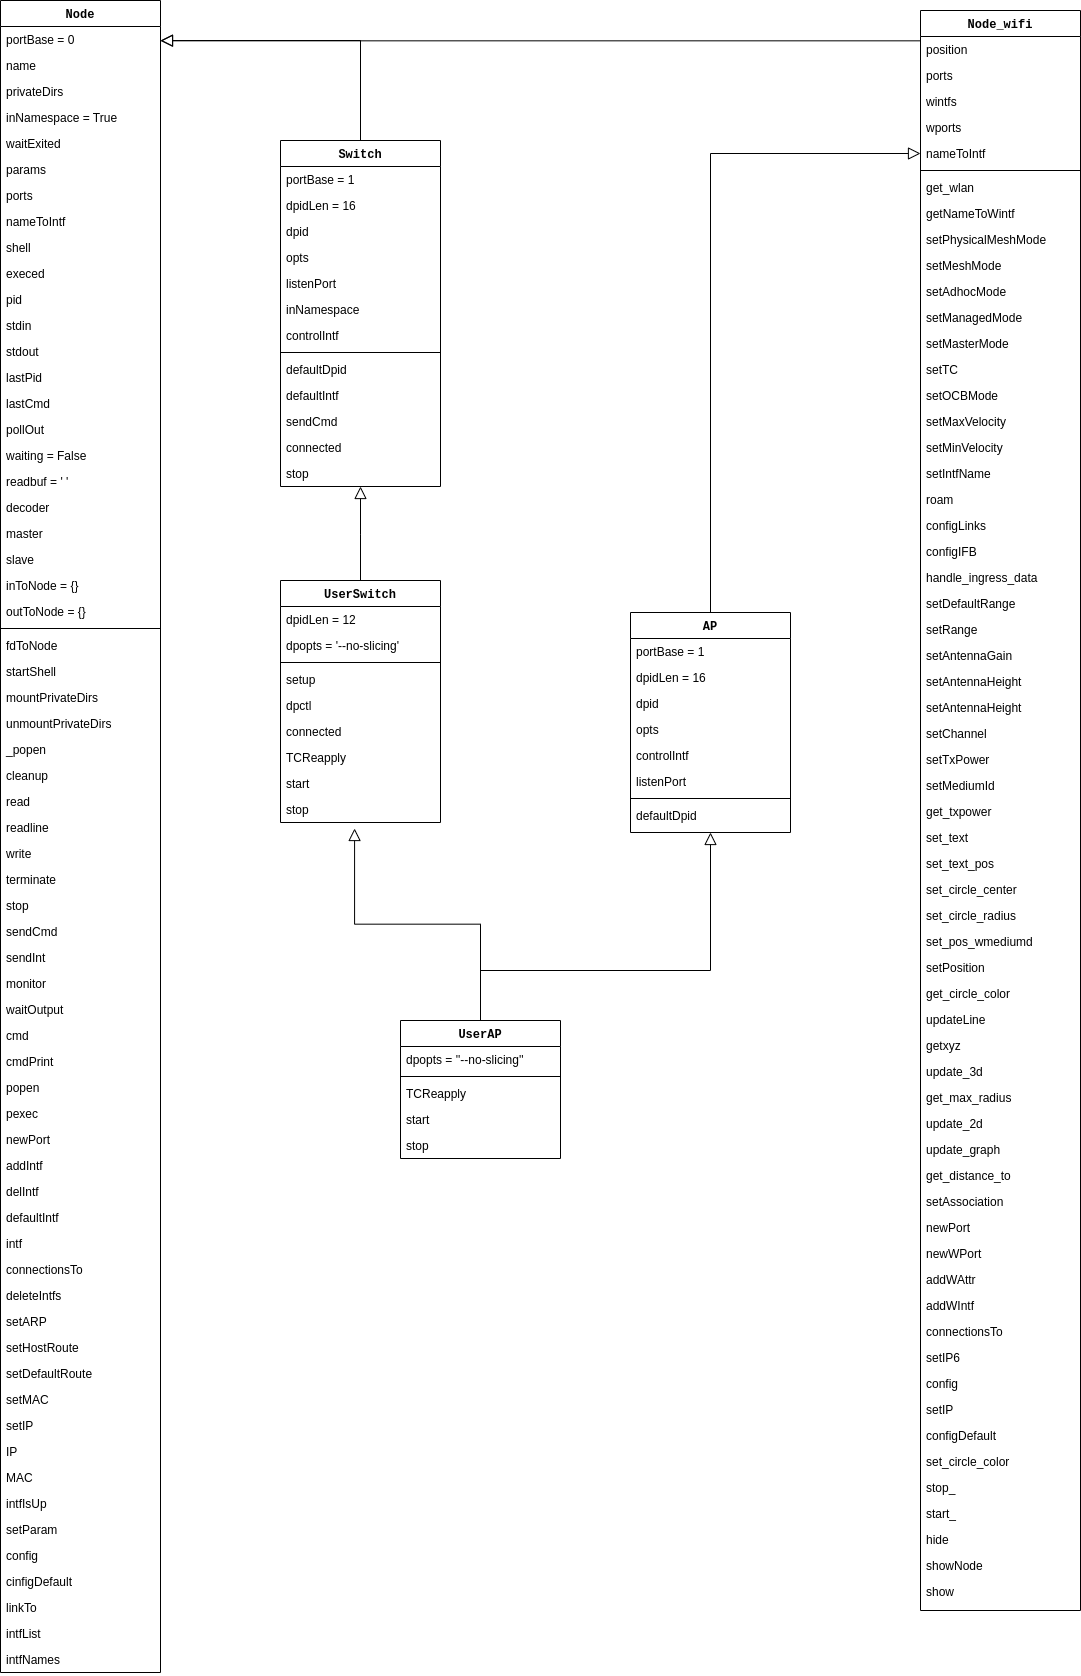
\includegraphics[width=0.8\textwidth]{archivos/img/analisis/userAP.png}
    \caption{Diagrama UML de la clase \texttt{UserAP}}
    \label{fig:userAP}
\end{figure}

Mencionar, que Mininet-Wifi redefine atributos que ya se encuentran en Mininet, como por ejemplo la longitud del identificador del \textit{datapath}. Muchos de los bugs encontrados entre los repositorios de las plataformas de emulación y el \gls{bofus}, se debe a incoherencias en la definición de las interfaces y a redefiniciones de parámetros como se ha podido encontrar. Por ello, para ver a bajo nivel como se ejecuta los binarios pertenecientes al \gls{bofus} se va a hacer una prueba de concepto lanzando una topología sencilla, y se va a estudiar las trazas de ejecución del mismo. Esto nos será de utilidad para poder comprender que comandos y llamadas al sistema se llevan a cabo para levantar una instancia de un software switch \gls{bofus}.\\
\\
La topología que se va a desplegar se puede apreciar en la figura \ref{fig:topoBasic}. Para lanzar dicha topología se tiene que lanzar un script de Python el cual se puede encontrar en el repositorio del \gls{tfm} (Sección \ref{sec:estadoArte_github}). A la par que se ejecuta el script de python que alberga la topología, se tiene que lanzar un controlador \gls{sdn} que le permita al software switch manejar correctamente los paquetes que atraviesen su \textit{datapath}. A continuación, en el bloque de código \ref{code:topoBasic}, se puede apreciar qué comandos se tienen que utilizar para  desplegar el escenario. \\

\begin{lstlisting}[language= bash, style=Consola, caption={Puesta en marcha del escenario básico},label=code:topoBasic]
    # Lanzamos el script que pone en marcha el medio inalambrico via Mininet-WiFi
    sudo python3 topo.py
   
    # Lanzamos el controlador (en otra terminal)
    ryu-manager ryu.app.simple_switch_13
\end{lstlisting}
\vspace{0.5cm}

Algún lector podría preguntarse en este punto como va a llevar se a cabo la comunicación entre el controlador \gls{sdn} y el \gls{bofus}. Dicha comunicación se producirá a través de la interfaz de red de \textit{loopback} de la Network namespace por defecto, donde el controlador de ryu estará escuchando en el puerto 6633, con una interfaz virtual de tipo \textit{tun} generada por el \gls{bofus} para llevar a cabo la conexión Openflow.  Para recolectar información sobre la traza de ejecución del script en Mininet-WiFi se debe poner el nivel de log a \textit{debug}.\\
\\

\begin{figure}[ht!]
    \centering
    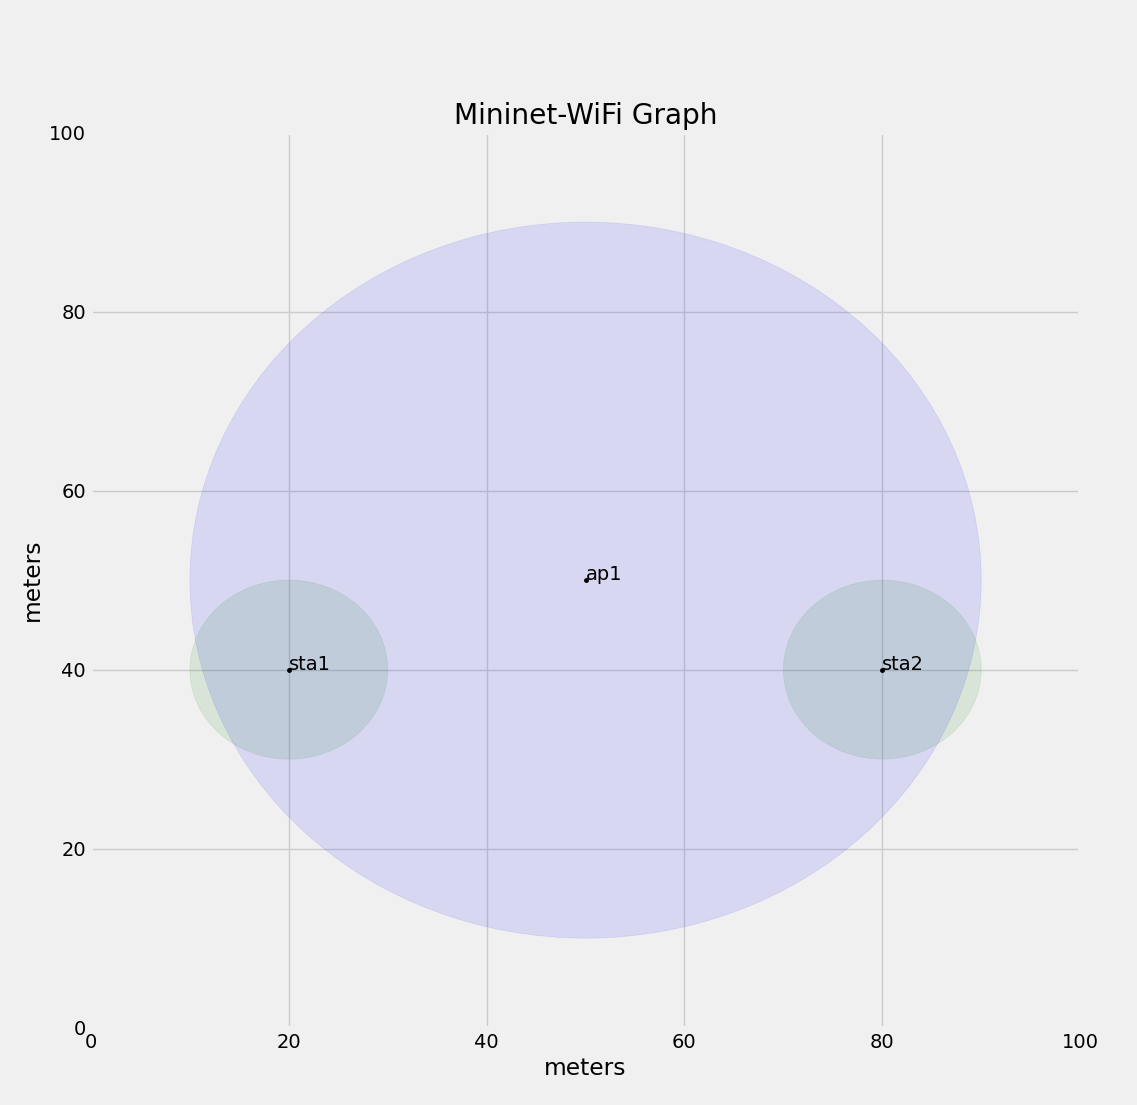
\includegraphics[width=0.7\textwidth]{archivos/img/analisis/topoBasic.png}
    \caption{Topología básica haciendo uso del \texttt{UserAP} (\gls{bofus})}
    \label{fig:topoBasic}
\end{figure}


A continuación, en el bloque de código \ref{code:trazatopobasic}, se puede apreciar la traza de ejecución de la topología básica. Dicha traza se ha limpiado y se han marcado las partes más importantes. Como se indicó anteriormente, esta traza es muy enriquecedora dado que nos permitirá a posteriori hacer nuestros propios escenarios a medida con topologías inalámbricas a bajo nivel. A lo largo de la traza, se podrán encontrar comentarios en verde que indican que operativas se están llevando a cabo en que parte.\\
\\

\begin{lstlisting}[language= bash, style=Consola, caption={Traza de la puesta en marcha del escenario básico},label=code:trazatopobasic]
    ### Primero se comprueba las caracteristicas del sistema sobre donde va a correr
    *** errRun: ['grep', '-c', 'processor', '/proc/cpuinfo'] 
    4
    0*** Setting resource limits
    *** Creating nodes
    *** Add Controller (Ryu) ***
    *** errRun: ['which', 'mnexec'] 
    /usr/bin/mnexec
    0*** errRun: ['which', 'ifconfig'] 
    /usr/sbin/ifconfig
    0_popen ['mnexec', '-cd', 'env', 'PS1=\x7f', 'bash', '--norc', '--noediting', '-is', 'mininet:c0'] 359891*** c0 : ('unset HISTFILE; stty -echo; set +m',)
    unset HISTFILE; stty -echo; set +m

    ### Se comprueba la conectividad con el controlador al puerto por defecto haciendole un telnet 
    *** c0 : ('echo A | telnet -e A localhost 6633',)
    Telnet escape character is 'A'.
    Trying 127.0.0.1...
    Connected to localhost.
    Escape character is 'A'.

    telnet> Connection closed.
    *** Add one UserAP ***
    *** errRun: ['which', 'mnexec'] 
    /usr/bin/mnexec
    0*** errRun: ['which', 'ip', 'addr'] 
    /usr/sbin/ip
    1_popen ['mnexec', '-cd', 'env', 'PS1=\x7f', 'bash', '--norc', '--noediting', '-is', 'mininet:ap1'] 359897*** ap1 : ('unset HISTFILE; stty -echo; set +m',)
    unset HISTFILE; stty -echo; set +m

    ### Se prepara el box del AP1 (El cual correrá el BOFUSS)
    added intf lo (0) to node ap1
    *** ap1 : ('ifconfig', 'lo', 'up')
    *** errRun: ['which', 'ofdatapath'] 
    /usr/local/bin/ofdatapath
    0*** errRun: ['which', 'ofprotocol'] 
    /usr/local/bin/ofprotocol

    ### Se prepara los boxes de las estaciones wifi
    *** Add two WiFi stations ***
    *** errRun: ['which', 'mnexec'] 
    /usr/bin/mnexec
    0*** errRun: ['which', 'ip', 'addr'] 
    /usr/sbin/ip
    1_popen ['mnexec', '-cdn', 'env', 'PS1=\x7f', 'bash', '--norc', '--noediting', '-is', 'mininet:sta1'] 359904*** sta1 : ('unset HISTFILE; stty -echo; set +m',)
    unset HISTFILE; stty -echo; set +m
    _popen ['mnexec', '-cdn', 'env', 'PS1=\x7f', 'bash', '--norc', '--noediting', '-is', 'mininet:sta2'] 359906*** sta2 : ('unset HISTFILE; stty -echo; set +m',)
    unset HISTFILE; stty -echo; set +m

    ### Se generan los radio taps emulados hacinedo uso del modulo del kernel mac80211_hwsim
    *** Configuring nodes
    Loading 3 virtual wifi interfaces
    Created mac80211_hwsim device with ID 0
    Created mac80211_hwsim device with ID 1
    Created mac80211_hwsim device with ID 2
    rfkill unblock 17

    ### Se cambian los nombres por defecto de las interfaces virtuales generadas a nombres 
    ### descriptivos que identifiquen a los nodos
    *** sta1 : ('ip link set wlan0 down',)
    *** sta1 : ('ip link set wlan0 name sta1-wlan0',)
    rfkill unblock 18
    *** sta2 : ('ip link set wlan1 down',)
    *** sta2 : ('ip link set wlan1 name sta2-wlan0',)
    *** ap1 : ('ip link set wlan2 down',)
    *** ap1 : ('ip link set wlan2 name ap1-wlan1',)
    *** ap1 : ('ip link set ap1-wlan1 up',)

    ### Se configura la interfaz virtual emulada wireless de la sta1
    added intf sta1-wlan0 (0) to node sta1
    *** sta1 : ('ip link set', 'sta1-wlan0', 'down')
    *** sta1 : ('ip link set', 'sta1-wlan0', 'address', '00:00:00:00:00:02')
    *** sta1 : ('ip link set', 'sta1-wlan0', 'up')
    *** sta1 : ('ip addr flush ', 'sta1-wlan0')
    *** sta1 : ('ip addr add 10.0.0.1/8 brd + dev sta1-wlan0 && ip -6 addr add 2001:0:0:0:0:0:0:1/64 dev sta1-wlan0',)
    *** sta1 : ('ip -6 addr flush ', 'sta1-wlan0')
    *** sta1 : ('ip -6 addr add', '2001:0:0:0:0:0:0:1/64', 'dev', 'sta1-wlan0')
    *** sta1 : ('ip link set lo up',)

    ### Se configura la interfaz virtual emulada wireless de la sta2
    added intf sta2-wlan0 (0) to node sta2
    *** sta2 : ('ip link set', 'sta2-wlan0', 'down')
    *** sta2 : ('ip link set', 'sta2-wlan0', 'address', '00:00:00:00:00:03')
    *** sta2 : ('ip link set', 'sta2-wlan0', 'up')
    *** sta2 : ('ip addr flush ', 'sta2-wlan0')
    *** sta2 : ('ip addr add 10.0.0.2/8 brd + dev sta2-wlan0 && ip -6 addr add 2001:0:0:0:0:0:0:2/64 dev sta2-wlan0',)
    *** sta2 : ('ip -6 addr flush ', 'sta2-wlan0')
    *** sta2 : ('ip -6 addr add', '2001:0:0:0:0:0:0:2/64', 'dev', 'sta2-wlan0')
    *** sta2 : ('ip link set lo up',)

    ### Se configura la interfaz virtual emulada wireless de la ap1 y el proceso
    ### de hostAPd
    added intf ap1-wlan1 (1) to node ap1
    *** ap1 : ('ip link set', 'ap1-wlan1', 'up')
    *** ap1 : ('ethtool -K', <WirelessLink ap1-wlan1>, 'gro', 'off')
    *** ap1 : ('ip link set', 'ap1-wlan1', 'down')
    *** ap1 : ('ip link set', 'ap1-wlan1', 'address', '00:00:00:00:00:01')
    *** ap1 : ('ip link set', 'ap1-wlan1', 'up')
    *** ap1 : ("echo 'interface=ap1-wlan1\ndriver=nl80211\nssid=new-ssid\nwds_sta=1\nhw_mode=g\nchannel=1\nctrl_interface=/var/run/hostapd\nctrl_interface_group=0' > mn359884_ap1-wlan1.apconf",)
    > > > > > > > *** ap1 : ('hostapd -B mn359884_ap1-wlan1.apconf ',)
    ap1-wlan1: interface state UNINITIALIZED->ENABLED
    ap1-wlan1: AP-ENABLED 
    *** ap1 : ('ip link set', 'ap1-wlan1', 'down')
    *** ap1 : ('ip link set', 'ap1-wlan1', 'address', '00:00:00:00:00:01')
    *** ap1 : ('ip link set', 'ap1-wlan1', 'up')

    ### Se configura la potencia y las caracteristicas intrinsecas de los enlaces 
    _popen ['mnexec', '-da', '359897', 'tc', 'qdisc', 'replace', 'dev', 'ap1-wlan1', 'root', 'handle', '2:', 'netem', 'rate', '54.0000mbit', 'latency', '1.00ms'] 360049*** ap1 : ('tc qdisc add dev ap1-wlan1 parent 2:1 handle 10: pfifo limit 1000',)
    *** sta1 : ('iw dev', 'sta1-wlan0 set txpower fixed 1400')
    *** sta2 : ('iw dev', 'sta2-wlan0 set txpower fixed 1400')
    *** ap1 : ('iw dev', 'ap1-wlan1 set txpower fixed 1400')
    *** Add links ***
    added intf sta1-wlan0 (0) to node sta1
    *** sta1 : ('ip link set', 'sta1-wlan0', 'up')
    *** sta1 : ('ethtool -K', <WirelessLink sta1-wlan0>, 'gro', 'off')
    *** executing command: tc qdisc show dev sta1-wlan0
    *** sta1 : ('tc qdisc show dev sta1-wlan0',)
    qdisc mq 0: root 
    qdisc fq_codel 0: parent :4 limit 10240p flows 1024 quantum 1514 target 5ms interval 100ms memory_limit 32Mb ecn drop_batch 64 
    qdisc fq_codel 0: parent :3 limit 10240p flows 1024 quantum 1514 target 5ms interval 100ms memory_limit 32Mb ecn drop_batch 64 
    qdisc fq_codel 0: parent :2 limit 10240p flows 1024 quantum 1514 target 5ms interval 100ms memory_limit 32Mb ecn drop_batch 64 
    qdisc fq_codel 0: parent :1 limit 10240p flows 1024 quantum 1514 target 5ms interval 100ms memory_limit 32Mb ecn drop_batch 64 
    at map stage w/cmds: ['%s qdisc add dev %s root handle 5:0 htb default 1', '%s class add dev %s parent 5:0 classid 5:1 htb rate 11.000000Mbit burst 15k']
    *** executing command: tc qdisc add dev sta1-wlan0 root handle 5:0 htb default 1
    *** sta1 : ('tc qdisc add dev sta1-wlan0 root handle 5:0 htb default 1',)
    *** executing command: tc class add dev sta1-wlan0 parent 5:0 classid 5:1 htb rate 11.000000Mbit burst 15k
    *** sta1 : ('tc class add dev sta1-wlan0 parent 5:0 classid 5:1 htb rate 11.000000Mbit burst 15k',)
    cmds: ['%s qdisc add dev %s root handle 5:0 htb default 1', '%s class add dev %s parent 5:0 classid 5:1 htb rate 11.000000Mbit burst 15k'] 
    outputs: ['', ''] 
    _popen ['mnexec', '-da', '359904', 'iwconfig', 'sta1-wlan0', 'essid', 'new-ssid', 'ap', '00:00:00:00:00:01'] 360059
    added intf sta2-wlan0 (0) to node sta2
    *** sta2 : ('ip link set', 'sta2-wlan0', 'up')
    *** sta2 : ('ethtool -K', <WirelessLink sta2-wlan0>, 'gro', 'off')
    *** executing command: tc qdisc show dev sta2-wlan0
    *** sta2 : ('tc qdisc show dev sta2-wlan0',)
    qdisc mq 0: root 
    qdisc fq_codel 0: parent :4 limit 10240p flows 1024 quantum 1514 target 5ms interval 100ms memory_limit 32Mb ecn drop_batch 64 
    qdisc fq_codel 0: parent :3 limit 10240p flows 1024 quantum 1514 target 5ms interval 100ms memory_limit 32Mb ecn drop_batch 64 
    qdisc fq_codel 0: parent :2 limit 10240p flows 1024 quantum 1514 target 5ms interval 100ms memory_limit 32Mb ecn drop_batch 64 
    qdisc fq_codel 0: parent :1 limit 10240p flows 1024 quantum 1514 target 5ms interval 100ms memory_limit 32Mb ecn drop_batch 64 
    at map stage w/cmds: ['%s qdisc add dev %s root handle 5:0 htb default 1', '%s class add dev %s parent 5:0 classid 5:1 htb rate 11.000000Mbit burst 15k']
    *** executing command: tc qdisc add dev sta2-wlan0 root handle 5:0 htb default 1
    *** sta2 : ('tc qdisc add dev sta2-wlan0 root handle 5:0 htb default 1',)
    *** executing command: tc class add dev sta2-wlan0 parent 5:0 classid 5:1 htb rate 11.000000Mbit burst 15k
    *** sta2 : ('tc class add dev sta2-wlan0 parent 5:0 classid 5:1 htb rate 11.000000Mbit burst 15k',)
    cmds: ['%s qdisc add dev %s root handle 5:0 htb default 1', '%s class add dev %s parent 5:0 classid 5:1 htb rate 11.000000Mbit burst 15k'] 
    outputs: ['', ''] 
    _popen ['mnexec', '-da', '359906', 'iwconfig', 'sta2-wlan0', 'essid', 'new-ssid', 'ap', '00:00:00:00:00:01'] 360065
    *** Build it ***
    *** Configuring nodes

    added intf sta1-wlan0 (0) to node sta1
    *** sta1 : ('ip link set', 'sta1-wlan0', 'up')
    *** sta1 : ('ethtool -K', <WirelessLink sta1-wlan0>, 'gro', 'off')

    added intf sta2-wlan0 (0) to node sta2
    *** sta2 : ('ip link set', 'sta2-wlan0', 'up')
    *** sta2 : ('ethtool -K', <WirelessLink sta2-wlan0>, 'gro', 'off')
    *** Start the controller ***
    *** Set controllers ***

    ### AQUÍ se lanza finalmente el BOFUSS
    *** ap1 : ('ofdatapath -i ap1-wlan1 punix:/tmp/ap1 -d 100000000001 --no-slicing 1> /tmp/ap1-ofd.log 2> /tmp/ap1-ofd.log &',)
    [1] 360070
    *** ap1 : ('ofprotocol unix:/tmp/ap1 tcp:localhost:6633 --fail=closed  --listen=punix:/tmp/ap1.listen 1> /tmp/ap1-ofp.log 2>/tmp/ap1-ofp.log &',)
    *** RUN Mininet-Wifis CLI ***
    *** Starting CLI:
    *** errRun: ['stty', 'echo', 'sane', 'intr', '^C'] 
\end{lstlisting}
\vspace{0.5cm}

De esta traza se quiere destacar, aparte de la gestión que lleva a cabo con las interfaces inalámbricas que se ha ido comentando a lo largo de la traza, es la ejecución de los binarios pertenecientes al software switch \gls{bofus}, \texttt{ofdatapath} y el \texttt{ofprotocol}. A continuación en el bloque \ref{code:bofussLaunch}, se dejan las líneas extraídas del bloque anterior.\\
\\

\begin{lstlisting}[language= bash, style=Consola, caption={Puesta en marcha del BOFUSS},label=code:bofussLaunch]
    # Binario del datapath 
    ofdatapath -i ap1-wlan1 punix:/tmp/ap1 -d 100000000001 --no-slicing 1> /tmp/ap1-ofd.log 2> /tmp/ap1-ofd.log 
   
    # Binario del agente de control
    ofprotocol unix:/tmp/ap1 tcp:localhost:6633 --fail=closed  --listen=punix:/tmp/ap1.listen 1> /tmp/ap1-ofp.log 2>/tmp/ap1-ofp.log 
\end{lstlisting}
\vspace{0.5cm}

Según se ha estudiado en la sección anterior \ref{sec:ana_bofuss} donde se ha estudiado la interfaz CLI del \gls{bofus}, podemos llegar a entender cada parámetro que Mininet-WiFi mediante la clase \texttt{UserAP} ha conseguido traducir del script de la topología básica a la llamada de los dos binarios del software switch.  De las dos llamadas a cada binario, se quiere mencionar que Mininet-WiFi por defecto suele mandar los logs del plano de datos y del agente de control al directorio temporal (\texttt{/tmp/}) de la distribución linux en cuestión, pero no solo los archivos de logs, también se ubican ahí los descriptores de archivos UNIX para intercomunicar \texttt{ofdatapath} y el \texttt{ofprotocol}.


%%%%%%%%%%%%%%%%%%%%%%%%%%%%%%%%%%%%%%%%%%%%%%%%%%%%%%%%%%%%%%%%%%%%%%%%%%%%%%%%%%%%%%%%%%%%%%%%%
\section{Análisis del entorno de depuración del \glsentryshort{bofus}}
\label{sec:ana_gdb}


%%%%%%%%%%%%%%%%%%%%%%%%%%%%%%%%%%%%%%%%%%%%%%%%%%%%%%%%%%%%%%%%%%%%%%%%%%%%%%%%%%%%%%%%%%%%%%%%%
